\documentclass[border=1pt]{standalone}
\usepackage{tikz}
\usepackage{luatexja}
\usetikzlibrary{decorations.pathmorphing}

\begin{document}
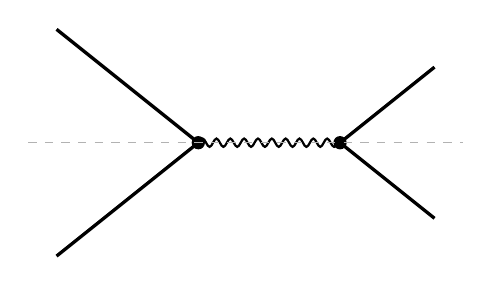
\begin{tikzpicture}[scale=1.2]
    % 粒子の飛来
    \draw[very thick] (-1.5, 1.2) -- (0,0);
    \draw[very thick] (-1.5, -1.2) -- (0,0);
    
    % 光子/グルーオンの交換（波線）
    \draw[thick, decoration={snake, amplitude=1.5pt, segment length=5pt}, decorate] (0,0) -- (1.5,0);
    
    % 散乱後の粒子
    \draw[very thick] (1.5,0) -- (2.5, 0.8);
    \draw[very thick] (1.5,0) -- (2.5, -0.8);
    
    % 頂点の強調
    \fill[black] (0,0) circle (2pt);
    \fill[black] (1.5,0) circle (2pt);
    
    % 数理的なアクセント（座標軸のメタファー）
    \draw[thin, dashed, black!30] (-1.8,0) -- (2.8,0);
\end{tikzpicture}
\end{document}
